\titleformat{\chapter}[display]
    {\normalfont\Large\bfseries}{\filleft\chaptertitlename\ \thechapter}{20pt}{\Huge}
    \chapter{Heurísticas y metaheurísticas para solucionar TSP}
        Las heurísticas y metaheurísticas permiten obtener resultados de manera más eficaces en la mayoría de los casos, no así más eficientes pues en ocasiones consumen incluso más recursos para trabajar. 
        
        Una heurística es una estrategia específica para problemas particulares, mientras que una metaheurística son enfoques generales y abstractos que pueden ser aplicados a más de un problema de optimización. 
        
            \section{Ant Colony Optimization ACO}
                
                Un algoritmo metaheurístico son métodos aproximados diseñados para resolver problemas de optimización combinatoria, en los que los heurísticos clásicos no son efectivos.
                La \textit{``Heurística de hormigas''} o de \textit{``colonia de hormigas''} \textbf{ACO} se basa en imitar a las feromonas producidas por las hormigas en un caso real, esto se refiere a que las hormigas producen feromonas al caminar y en base a esta se establecen los caminos más cortos. Es uno de los ``\textit{algoritmos bioinspirados}" mas populares.
                \newline
                \newline
                En relación a lo anterior, existe una primera hormiga que establece este patrón, el resto se guía por las feromonas dejadas en el camino. Si bien todas propagan dichas feromonas las mayormente concentradas o con más residuos (menos tiempo desde qué pasó la primera hormiga) será la que determine la ruta preferente. Dentro del \textit{paper} \parencite{ACO} se entrega un buen ejemplo de la manera de trabajar de las hormigas, así como casos de aplicación, ventajas y desventajas. En definitiva, un buen resumen.
                \newline
                \newline
                Esta Heurística plantea una \textit{``información heurística''} la cual se conforma por la preferencia de las hormigas para moverse de un nodo a otro. Esta información no es modificada durante la ejecución del algoritmo. Por otro lado, está la información que mide la deseabilidad de escoger un nodo u otro imitando a las hormigas cuando escogen una feromona, esto se va modificando continuamente con las decisiones que van encontrando los insectos.  
                \newline
                \newline
                Como se menciona en un inicio, los algoritmos \textbf{ACO} son procesos iterativos, en la que hormigas artificiales construyen soluciones de manera probabilística guiándose por feromonas del mismo tipo, las cuales buscan emular la realidad. La regla probabilística de este método dentro del \textbf{TSP} puede ser definida dependiendo del problema, como en el caso de \parencite{ACOTRANSPORTE}, donde se plantea una solución para un problema de transporte de paquetes con muchos orígenes a muchos destinos con varios \textit{hubs} (lugar donde se reúnen las cargas de mercancías).
                \newline
                \newline
                Dentro de este documento se aplica \textbf{ACO} para resolver un problema de distribución de paquetes. En él se decide dividir el problema en dos subtipos con el fin de facilitar su desarrollo, el subproblema ``\textit{d-h}'' y subproblema \textit{``d-h-p''}, si bien ambos se resuelven mediante la metaheurística en cuestión lo que los diferencia es que \textit{``d-h-p''} puede realizar\textit{ peddling}, que en el contexto de distribución de paquetería significa que puede realizar paradas múltiples.  
                \newline
                \newline
                Dentro de las conclusiones del documento se establece que para ejemplos con uno o dos \textit{hubs} el heurístico resuelve el subproblema \textit{``d-h''} de manera exacta mientras que con tres \textit{hubs} el error medio encontrado no supera el 3\%. En cuanto al subproblema \textit{``d-h-p''} el máximo error relativo medio alcanzado es de 1.2\% para ejemplos con 7 orígenes y 2 destinos.  
                \newline
                \newline
                En general, el documento demuestra mediante aplicaciones la ventaja de utilizar \textbf{ACO} para resolver problemas con muchos destinos o nodos en comparación a métodos tradicionales, permitiendo encontrar la distancia total más corta que se debe recorrer para visitar las ciudades. 
            \section{Algoritmo GRASP}
                El algoritmo \textbf{GRASP} (\textit{Greedy Randomized Adaptive Search Procedure}) es una combinación de dos técnicas utilizadas, elementos de construcción de soluciones y búsqueda local. Consiste en dos fases principales: Construcción de soluciones y mejora iterativa. 
                \newline
                \newline
                En la fase de construcción de soluciones, se utiliza un algoritmo \textit{greedy ávido} para construir soluciones iniciales.  Una función de evaluación ávida se refiere a una función que asigna un valor a cada posible solución en función de lo ``prometedora'' que parece ser desde un punto de vista local.            
                \newline
                \newline
                De esta manera se toman decisiones localmente óptimas en cada paso, eligiendo la mejor opción disponible según un criterio especifico. Sin embargo, se considera una metaheurística ya que para evitar quedarse atascado en óptimos locales, se introduce un componente aleatorio en la selección, lo que permite explorar distintas posibles soluciones. 
                \newline
                \newline                                  
                Una vez que se termina la primera fase, se pasa a la fase de mejora iterativa. En esta fase, como su nombre lo indica, se realizan mejoras continuamente aplicando operadores de búsqueda local para explorar el espacio de soluciones vecinas.  
                \newline
                \newline
                La búsqueda local se centra en hacer pequeños cambios en la solución actual y evaluar su impacto en la función objetivo. Si se encuentra una mejora, se actualiza la solución actual y se continúa iterando hasta que no se pueda encontrar una mejora adicional.  
                \newline
                \newline
                Al ser una metaheurística tiene múltiples aplicaciones, entre ella está la implementación en problemas de cortes de guillotina. 
                \newline
                \newline
                Este problema ha sido ampliamente estudiado en las dos últimas décadas, debido a su gran aplicabilidad en sectores productivos tales como la industria del papel, vidrio, metal y madera.\parencite{GRASPGUILLOTINA}
                \newline
                \newline
                Otra de las aplicaciones de esta metaheurística es para realizar búsqueda de subconjuntos o búsqueda de combinatorias. Como en el caso de \parencite{GRASPFINANCIERO}, dentro de este folio se utiliza GRASP para predecir el quiebre o solvencia empresarial, buscando las ratios financieras de una cierta cantidad de empresas. 
                \newline
                \newline
                En general, este documento compara la precisión de \textbf{GRASP} con el método constructivo determinístico (modelo clásico) y el \textit{método ávido aleatorio} (GRASP sin fase de mejora iterativa) y demuestra la superioridad de la metaheurística. 
                \newline
                \newline
                Para el caso del TSP se utiliza un procedimiento similar, se generan soluciones iniciales de manera greedy, puede ser incluso utilizando ACO para recorrer todas las ciudades, siempre agregando un elemento aleatorio para evitar los óptimos locales. Luego ir mejorando la solución mediante búsqueda local, realizando varias iteraciones. 
                
            \section{Simulated Annealing SA}
                El nombre e inspiración de \textit{Simulated Annealing} viene del proceso de reconocido del acero y cerámicas, una técnica que consiste en calentar y luego enfriar lentamente el material para variar sus propiedades físicas.\parencite{WikipediaTSP}
                \newline
                \newline
                Esto quiere decir que a medida que el algoritmo se ejecuta, se aceptan soluciones subóptimas en busca de una solución óptima global.  
                \newline
                \newline
                El proceso de búsqueda del algoritmo se realiza mediante una función que mide la calidad de la solución en términos del objetivo de optimización. Durante la ejecución del algoritmo, se generan soluciones vecinas mediante movimientos o cambios en la solución actual. Si una solución vecina es mejor que la solución actual, se acepta como la nueva solución. Un aspecto a destacar es que también se aceptan soluciones peores en función de una probabilidad que disminuye a mediad que el algoritmo avanza. Esto último permite evitar quedar atrapado en óptimos locales. 
                \newline
                \newline
                Por ultimo, SA (\textit{Simulated Annealing}) de la misma manera que GRASP es capaz de adaptarse a múltiples problemas de optimización, es por esta razón que es considerada metaheurística. 
    
            \section{Implementaciones en código}
                Si bien los algoritmos presentados anteriormente son mas eficaces que metodologías tradicionales, es importante recordar que estos algoritmos son, en la mayoría de los casos bastante más eficaces que resolverlos por enumeración exhaustiva, por ejemplo. Asimismo, esto no significa que dejen de ser de NP-Completos lo que implica que su eficiencia seguirá siendo limitada, en resumen, mayor costo computacional (menor eficiencia) y menos tiempo de cómputo (mayor eficacia). 
                \newline
                \newline
                Por otro lado, para probar y comparar rendimientos entre algoritmos se plantean distintos códigos, todos ellos documentados en el repositorio \parencite{RepoTSP} y elaborados en \textbf{Julia}. Dichos resultados se pueden ver representados en el Cuadro 3.1.
                \newline
                \begin{table}[ht]
                  \centering
                  \caption{Comparación de resultados}
                  \adjustbox{max width=\textwidth}{
                  \begin{tabular}{|l|l|l|l|l|l|}
                      \hline
                      \textbf{Algoritmo} & \textbf{Segundos} & \textbf{K Locaciones} & \textbf{MiB} & \textbf{Porcentaje} & \textbf{Costo del mejor recorrido} \\ \hline
                      GRASP              & 0.128384         & 23.47                 & 1.630        & 98.80\%            & 1.414                \\ \hline
                      Simulated Annealing & 0.053644         & 20.20                 & 1.336        & 99.28\%            & 5.656                  \\ \hline
                      ACO                & 1.384717         & 371.77                & 14.724       & 98.93\%            & 5.656                 \\ \hline
                    \end{tabular}
                  }
                  \label{tab:resultados}
                \end{table}
                \newline
                Como se puede apreciar, por cada uno de los algoritmos implementados se obtiene una columna con sus respectivos valores, la primera columna es del \textit{tiempo de ejecución en segundos}, a continuación están las \textit{k locaciones} que son el numero de asignaciones de memoria, la \textit{cantidad de memoria en mebibytes}, luego esta el \textit{porcentaje de tiempo de recursos} y finalmente el \textit{costo del mejor recorrido.} 
                \newline
                \newline
                Con los valores presentados en el Cuadro 3.1 se pueden llegar a las siguientes conclusiones:
                \begin{enumerate}
                    \item La heurística \textbf{SA} (\textit{Simulated Annealing}) encuentra una solución en menos tiempo que las otras dos heurísticas, por el contrario\textbf{ ACO} (\textit{Ant Colony Optimization}) es la que mas tiempo tarda en hallar una respuesta. Esto puede ser originado por la mayor complejidad de \textbf{ACO}, pues requiere de mas cálculos y operaciones en cada iteración. También podría ser por la cantidad de hormigas asignadas.
                    \item Tanto la \textbf{SA} como el algoritmo \textbf{GRASP} tienen \textit{K locaciones} similares, no así \textbf{ACO}, pues esta bastante mas lejos. Esto es debido a la naturaleza del algoritmo como tal, pues \textbf{ACO} requiere almacenar y actualizar las matrices que representan a las feromonas.
                    \item En cuanto a la \textit{memoria utilizada} por razones similares al punto 2, las matrices de feromonas, matrices de visibilidad, entre otras cosas el algoritmo \textbf{ACO} es el que mas consume de los tres y el que tiene valores mas alejados. 
                    \item Para el\textit{ porcentaje de tiempos de recursos} mas alto se lo lleva el \textbf{SA}, este valor quiere decir que dicho algoritmo pasó mas tiempo en fase de compilación  que en la ejecución real. Por el contrario, el que mas tiempo llevo compilar fue el \textbf{GRASP}, aunque por valores ligeramente superiores.
                    \item Por ultimo, el que obtuvo un menor \textit{costo del mejor recorrido} fue el algoritmo \textbf{GRASP} que si bien tarda un par de segundos mas en trabajar, es menos costoso, es decir, al menos para este caso particular \textbf{GRASP} es el mas eficaz y \textbf{SA} el mas eficiente.
                \end{enumerate}                      
                Si bien los algoritmos presentados anteriormente son más eficaces que metodologías tradicionales, esto no significa que dejen de ser de \textit{NP-Completos} lo que implica que su eficiencia seguirá siendo limitada.
            \subsection{Resultados obtenidos}
                Con el fin de verificar los puntos previamente señalados, se vuelven a iterar los algoritmos, en esta ocasión se realizan 100 iteraciones por cada uno. De esta manera, se obtienen gráficos que permiten visualizar el rendimiento en cada una de las áreas previamente señaladas, es decir, \textit{tiempo de ejecución en segundos}, \textit{k locaciones}, \textit{cantidad de memoria en mebibytes}, \textit{porcentaje de recursos utilizados} y \textit{costo del mejor recorrido}.
                \newline
                \newline
                Dentro de las métricas que se logran obtener, destacan la \textit{gráfica de tiempo de ejecución} y de \textit{asignaciones}, \textit{Figura 3.1} y \textit{3.2} respectivamente.
                \newline
                \begin{figure}[ht]
                    \centering
                        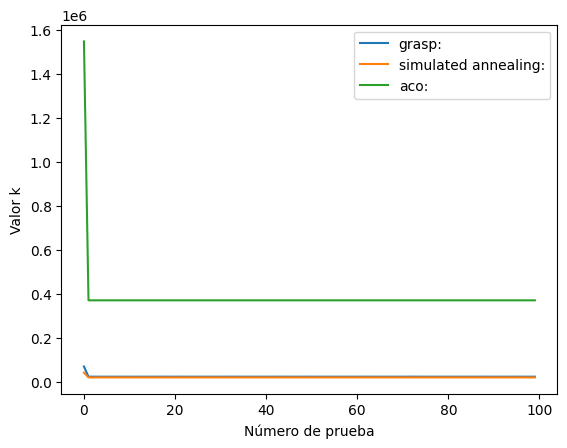
\includegraphics[scale=0.8]{imgs/Grafico_k.png}
                        \caption{Gráfico de valores k en cada iteración}
                        \label{Ilustracion 2}
                \end{figure}                
                \newline
                La \textit{Figura 3.1} permite ver comparar la eficacia de cada uno de los algoritmos, donde se determina que al menos para esta prueba el \textit{Simulated Annealing} es constantemente mas eficaz que los otros dos algoritmos. Por el contrario, el \textit{Ant Colony Optimization} es mucho mas lento en comparación.
                \newpage
                \begin{figure}[ht]
                    \centering
                        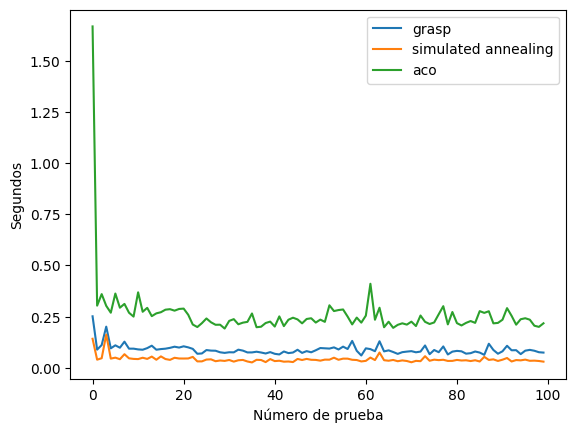
\includegraphics[scale=0.8]{imgs/Grafico_s.png}
                        \caption{Gráfico de tiempo de ejecución en cada iteración}
                        \label{Ilustracion 3}
                \end{figure}                
                Por otro lado, la \textit{Figura 3.2} muestra la cantidad de asignaciones que realiza cada uno de los algoritmos. El resultado obtenido, en esta ocasión es esperable, puesto que el algoritmo \textbf{ACO} debe realizar tales asignaciones para su funcionamiento. Por el contrario, tanto \textbf{GRASP} como \textbf{SA} realizan, aparentemente, la misma cantidad de asignaciones. En definitiva, mucho más eficientes en comparación.
                \newline
                \newline
                En general, los gráficos que generó este experimento permiten llegar a la conclusión de que al menos para casos pequeños el algoritmo consume una gran cantidad de recursos para llegar a una solución, esto debido a su propia naturaleza, puesto que debe utilizar memoria tanto como para guardar recorridos anteriores (en caso de tener que volver) como para ser ejecutado y esto en cada iteración.
